% ANUfinalexam.tex (Version 2.0)
% ===============================================================================
% Australian National University Final Exam LaTeX template.
% 2004; 2009, Timothy Kam, ANU School of Economics
% Licence type: Free as defined in the GNU General Public Licence: http://www.gnu.org/licenses/gpl.html

\documentclass[a4paper,12pt,fleqn]{article}
\usepackage[]{standalone}
%\usepackage[subpreambles=false]{standalone}
\setlength{\parindent}{0em}
\usepackage{amsmath}
\usepackage{enumitem}
\usepackage{fancyhdr}
\usepackage{siunitx}
\usepackage{amsmath}
\usepackage{float}
\usepackage[caption = false]{subfig}
\usepackage{graphicx}
\usepackage{tikz}
\usepackage{pgfplots}
\usetikzlibrary{arrows,shapes,positioning,calc,intersections}
\usetikzlibrary{decorations.markings}
\tikzstyle arrowstyle=[scale=1]
\tikzstyle directed=[postaction={decorate,decoration={markings,
    mark=at position .65 with {\arrow[arrowstyle]{stealth}}}}]
\tikzstyle reverse directed=[postaction={decorate,decoration={markings,
    mark=at position .65 with {\arrowreversed[arrowstyle]{stealth};}}}]
\usepackage{import}
\usepackage{comment}

% Unit definitions %%%%%%%%%%%%%%%%%%%%%%%%%%%%%%%%%%

\DeclareSIUnit\kilowatthour{kWh}
\DeclareSIUnit\megawatthour{MWh}
\DeclareSIUnit\kilowattpeak{kW_P}
\DeclareSIUnit\kVA{kVA}
\DeclareSIUnit\kVAR{kVAR}
\DeclareSIUnit\rpm{rpm}
\DeclareSIUnit\year{y}
\DeclareSIUnit\north{N}
\DeclareSIUnit\south{S}
\DeclareSIUnit\second{s}
\DeclareSIUnit\pence{p}
\DeclareSIUnit\pound{£}


% Insert your course information here %%%%%%%%%%%%%%%%%%%%%%%%%%%%%%%%%%

\newcommand{\institution}{CORNWALL COLLEGE}
\newcommand{\titlehd}{BSc Renewable Energy and Carbon Management}
\newcommand{\examtype}{Referral Exam}
\newcommand{\examdate}{Academic Year 2014-2015}
\newcommand{\examcode}{CORC2089}
\newcommand{\examtitle}{Wind Energy}
\newcommand{\readtime}{15 Minutes}
\newcommand{\writetime}{Two Hours}
\newcommand{\materials}{Non-programmable Calculators; Formula Sheet}
\newcommand{\middlewords}{Exam continues on next page}
\newcommand{\lastwords}{End of Exam}


%%%%%%%%%%%%%%%%%%%%%%%%%%%%%%%%%%%%%%%%%%%%%%%%%%%%

%\setcounter{MaxMatrixCols}{10}
\newtheorem{theorem}{Theorem}
\newtheorem{acknowledgement}[theorem]{Acknowledgement}
\newtheorem{algorithm}[theorem]{Algorithm}
\newtheorem{axiom}[theorem]{Axiom}
\newtheorem{case}[theorem]{Case}
\newtheorem{claim}[theorem]{Claim}
\newtheorem{conclusion}[theorem]{Conclusion}
\newtheorem{condition}[theorem]{Condition}
\newtheorem{conjecture}[theorem]{Conjecture}
\newtheorem{corollary}[theorem]{Corollary}
\newtheorem{criterion}[theorem]{Criterion}
\newtheorem{definition}[theorem]{Definition}
\newtheorem{example}[theorem]{Example}
\newtheorem{exercise}[theorem]{Exercise}
\newtheorem{lemma}[theorem]{Lemma}
\newtheorem{notation}[theorem]{Notation}
\newtheorem{problem}[theorem]{Problem}
\newtheorem{proposition}[theorem]{Proposition}
\newtheorem{remark}[theorem]{Remark}
\newtheorem{solution}[theorem]{Solution}
\newtheorem{summary}[theorem]{Summary}
\newenvironment{proof}[1][Proof]{\noindent\textbf{#1.} }{\ \rule{0.5em}{0.5em}}

% ANU Exams Office mandated margins and footer style
\setlength{\topmargin}{0cm}
\setlength{\textheight}{9.75in}
\setlength{\oddsidemargin}{0.0in}
\setlength{\evensidemargin}{0.0in}
\setlength{\textwidth}{16cm}
\pagestyle{fancy}
\lhead{} 
\chead{} 
\rhead{} 
\lfoot{} 
\cfoot{\footnotesize{Page \thepage \ of \pageref{finalpage} -- \titlehd \ (\examcode)}} 
\rfoot{} 

% DEPRECATED: ANU Exams Office mandated margins and footer style
%\setlength{\topmargin}{0cm}
%\setlength{\textheight}{9.25in}
%\setlength{\oddsidemargin}{0.0in}
%\setlength{\evensidemargin}{0.0in}
%\setlength{\textwidth}{16cm}
%\pagestyle{fancy}
%\lhead{} %left of the header
%\chead{} %center of the header
%\rhead{} %right of the header
%\lfoot{} %left of the footer
%\cfoot{} %center of the footer
%\rfoot{Page \ \thepage \ of \ \pageref{finalpage} \\
%       \texttt{\examcode}} %Print the page number in the right footer

\renewcommand{\headrulewidth}{0pt} %Do not print a rule below the header
\renewcommand{\footrulewidth}{0pt}


\begin{document}

% Title page

\begin{center}
%\vspace{5cm}
\large\textbf{\institution}
\end{center}
\vspace{1cm}

\begin{center}
\textit{ \examtype -- \examdate}
\end{center}
\vspace{1cm}

\begin{center}
\large\textbf{\titlehd}
\end{center}

\begin{center}
\large\textbf{\examcode}
\end{center}
\begin{center}
\large\textbf{\examtitle}
\end{center}
\vspace{4cm}
\vspace{4cm}

\begin{center}
%\textit{Reading Time: \readtime}
\end{center}
\begin{center}
\textit{Time Allowed:  \writetime}
\end{center}
\begin{center}
\textit{Permitted Materials: \materials}
\end{center}

% End title page
\newpage
\textbf{Formulae and constants}
\newline\newline
$\mathrm{Star: }V_\mathrm{L}=\sqrt{3}V_\mathrm{P}$
\newline\newline
$\mathrm{Star: }I_\mathrm{L}=I_\mathrm{P}$
\newline\newline
$\mathrm{Delta: }V_\mathrm{L}=V_\mathrm{P}$
\newline\newline
$\mathrm{Delta: }I_\mathrm{L}=\sqrt{3}I_\mathrm{P}$
\newline\newline
$P=3V_\mathrm{P}I_\mathrm{P}=\sqrt{3}V_\mathrm{L}I_\mathrm{L}$
\newline\newline
$\mathrm{rpm}=\dfrac{60f}{n_\mathrm{P}}$
\newline\newline
$\mathrm{Tip\ speed\ }u=\dfrac{\mathrm{rpm}}{60}\cdot\pi D$
\newline\newline
$\mathrm{TSR\ }\lambda=\dfrac{u}{v}$
\newline\newline
$P=\omega\tau$
\newline\newline
$P=\dfrac{1}{2}\rho Av^3$

\newpage

\begin{quote}
    \begin{center}
        \textit{Answer any \textbf{TWO} questions.}
    \end{center}
\end{quote}

\begin{quote}
    \begin{center}
        \textit{All questions carry equal weighting.}
    \end{center}
\end{quote}

\begin{quote}
    \begin{center}
        \textit{There is a total of \textbf{26} marks.}
    \end{center}
\end{quote}

\begin{quote}
    \begin{center}
        \textit{Answers should contain clear mathematical workings where appropriate.}
    \end{center}
\end{quote}

\newpage


\paragraph{\textbf{Question 1: (13 marks)}}


The power and power coefficient of a wind turbine as a function of wind speed and the annual energy production as a function of mean wind
speed at hub height are shown in Figure \ref{figure:q1} ((a) and (b))

\begin{figure}
    \subfloat[Power $P$ (circles, left axis) and power coefficient $c_\mathrm{P}$ (squares, right axis) of the wind turbine as a function of wind speed]{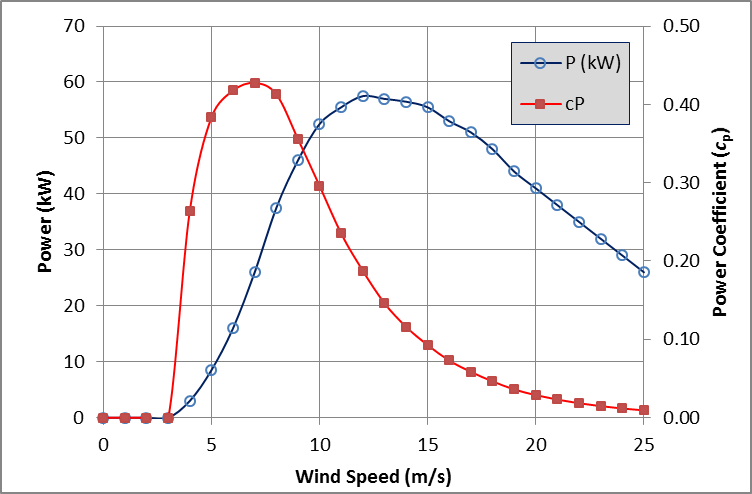
\includegraphics[width=0.8\textwidth]{./figures/E3120.tex}}\\
    \subfloat[Annual energy production of the turbine as a function of mean wind speed at hub height]{\includegraphics[width=0.8\textwidth]{./figures/AEP.tex}} \\
    \subfloat[Wind speed duration curve at turbine site]{\includegraphics[width=0.8\textwidth]{./figures/duration.tex}} \\
    %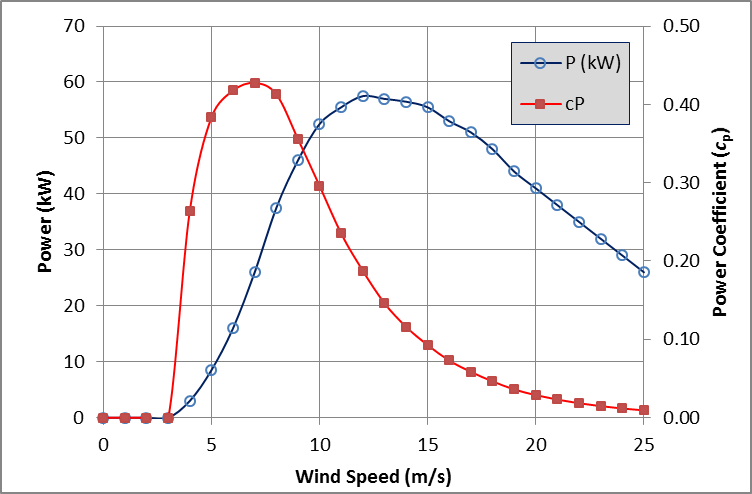
\includegraphics[width=0.8\textwidth]{./figures/E3120.tex}
    %\newline\newline
    %\includegraphics[width=0.8\textwidth]{./figures/AEP.tex}
   %\newline\newline
    %\includegraphics[width=0.8\textwidth]{./figures/duration.tex}
    \caption{For use with Question One}

\label{figure:q1}
\end{figure}
\newline
The turbine is at a site where wind speeds have been monitored and where the wind speed duration curve at the hub height of the turbine is as shown in 
Figure \ref{figure:q1} (c). 
The mean wind speed at this height is \SI{6.1}{\metre\per\second}

\begin{enumerate} [resume,label=\alph*)]
\item \lbrack\ 3 marks ] \ Wind speed atlases exist for the UK, so why would the wind speeds at the site have been monitored?
\item \lbrack\ 1 mark ] \ At what wind speed is the wind turbine most efficient?
\item \lbrack\ 1 mark ] \ At what wind speed does the wind turbine produce most power?
\item \lbrack\ 2 marks ] \ What is the median wind speed at this site?
\item \lbrack\ 2 marks ] \ For what proportion of the time is the wind turbine not generating?
\item \lbrack\ 2 marks ] \ For what proportion of the time is the wind turbine generating \SI{50}{\kilo\watt} or more?
\item \lbrack\ 2 marks ] \ If the rated power of this turbine is \SI{50}{\kilo\watt}, what is its capacity factor at this site?
\end{enumerate}

\begin{center}
\vspace{3cm}
--------- \textit{\middlewords} ---------
\end{center}
\newpage

\paragraph{\textbf{Question 2: (13 marks)}}
Figure \ref{figure:q2} shows a section through a rotor blade of the wind turbine of Question 1, at a point where the forward velocity
 of the leading edge is $u$, and at a time when the wind speed is $v$.
\begin{figure}
\centering
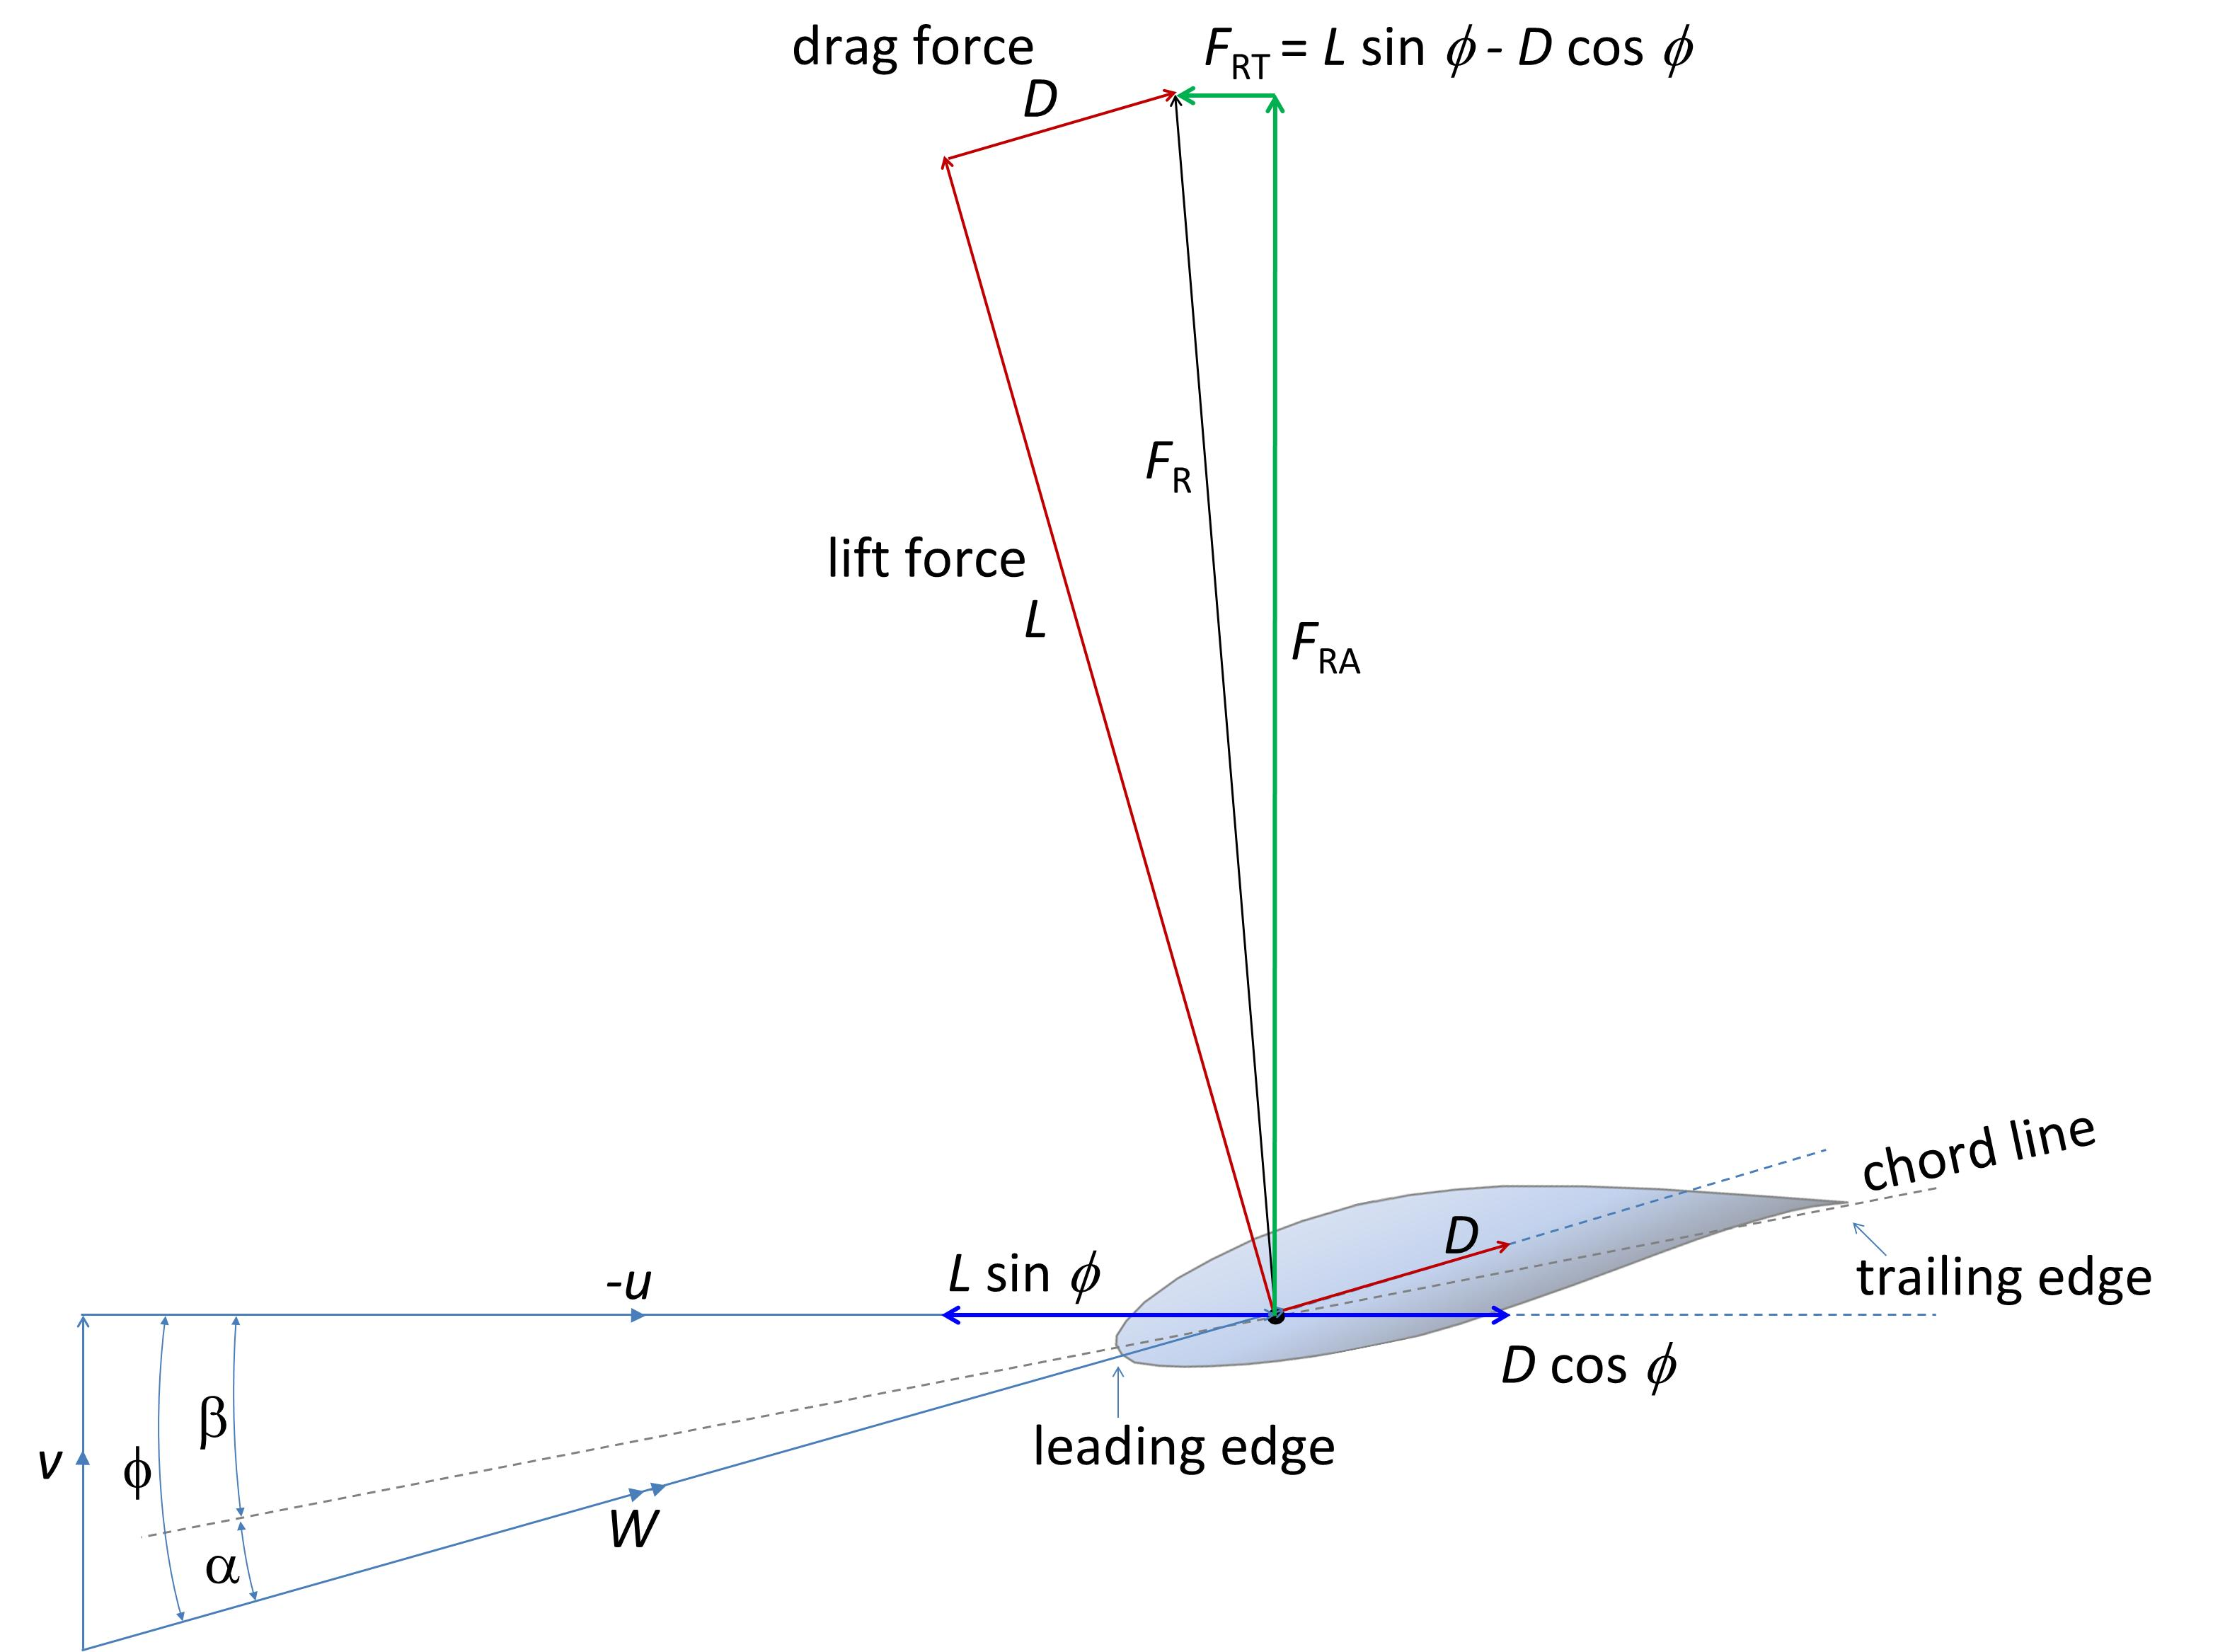
\includegraphics[width=0.85\textwidth]{./figures/vectors}
\caption{Section through foil of turbine}
\label{figure:q2}
\end{figure}

\begin{enumerate} [label=\alph*)]
\item \lbrack\ 3 marks ] \ Identify from this diagram the quantities that represent the 
    \begin{enumerate} [label=\roman*)]
        \item pitch angle
        \item angle of attack
        \item apparent velocity
    \end{enumerate}
\item \lbrack\ 4 marks ] \ Draw a sketch to show that if the wind speed were to increase, then the angle of attack would also increase.
\item \lbrack\ 3 marks ] \ If that happened, what could be done to reduce the angle of attack back to its original value?
\item \lbrack\ 3 marks ] \ Explain why the rotor blade stalls if the angle of attack becomes too large.
\end{enumerate}

\begin{center}
\vspace{3cm}
--------- \textit{\middlewords} ---------
\end{center}
\newpage

\paragraph{\textbf{Question 3: (13 marks}}
A \SI{6}{\kilo\watt} wind turbine on a small holding generates \SI{10000}{\kilowatthour} per year. The household uses \SI{4000}{\kilowatthour}
per year and \SI{8000}{\kilowatthour} per year is exported. The Feed-in tariff (FiT) for this turbine when commissioned was \SI{23}{\pence\per\kilowatthour},
the export tariff was \SI{4.7}{\pence\per\kilowatthour} and the import tariff is \SI{15}{\pence\per\kilowatthour}. 
The cost of the turbine was \SI{25000}[\pounds]{}.
\begin {enumerate} [label=\alph*)]
\item \lbrack\ 3 marks ] \ What is the annual income from the FiT?
\item \lbrack\ 3 marks ] \ By how much is the annual electricity bill of the small holding reduced because of the turbine?
\item \lbrack\ 3 marks ] \ Estimate the simple pay-back time of this turbine.
\item \lbrack\ 2 marks ] \ If discounting is taken into account, what impact would that have on the pay-back time as calculated in the previous part?
\item \lbrack\ 2 marks ] \  What could the owners do to reduce this payback time?
\end{enumerate}


\paragraph{\textbf{Question 4: (13 marks)}}
Wind power is widely regarded as a low-carbon source of electricity. Briefly outline the circumstances (if any) under which this is true.
A good answer will demonstrate knowledge of the actual carbon intensity of wind-produced electricity, how this compares to the carbon intensity 
of electricity from other sources and of the factors that most contribute to it.


\begin{center}
\vspace{3cm}
--------- \textit{\lastwords} ---------
\end{center}


\label{finalpage}

%\begin{comment}

\newpage
\paragraph{\textbf{Solutions} \ }
\paragraph{\textbf{Solutions to Question 1: (13 marks)}}

The power and power coefficient as a function of wind speed and the annual energy production as a function of mean wind
speed at hub height are shown in Figure \ref{figure:q1} (top and middle)

The turbine is at a site where wind speeds have been monitored and where the wind speed duration curve at the hub height of the turbine is as shown in 
Figure \ref{figure:q1} (bottom). 
The mean wind speed at this height is \SI{6.1}{\metre\per\second}

\begin{enumerate} [resume,label=\alph*)]
\item \lbrack\ 3 marks ] \ Wind speed atlases exist for the UK, so why would the wind speeds at the site have been monitored?\par
Atlases generally have resolution of \SI{1}{\km\squared} within which wind speeds may vary considerably.
\item \lbrack\ 1 mark ] \ At what wind speed is the wind turbine most efficient?\par
\SI{7}{\metre\per\second}
\item \lbrack\ 1 mark ] \ At what wind speed does the wind turbine produce most power?\par
\SI{13}{\metre\per\second}
\item \lbrack\ 2 mark ] \ What is the median wind speed at this site?\par
=wind speed exceeded 50\% of the time, = \SI{6}{\metre\per\second}
\item \lbrack\ 2 marks ] \ For what proportion of the time is the wind turbine not generating?\par
Cut off wind speed $\approx \SI{3}{\metre\per\second}$ Wind speed less than this about 12% of time.
\item \lbrack\ 2 marks ] \ For what proportion of the time is the wind turbine generating \SI{50}{\kilo\watt} or more?\par
Require $v\geq\SI{9}{\metre\per\second}$, occurs about 12\% of time
\item \lbrack\ 2 marks ] \ If the rated power of this turbine is \SI{50}{\kilo\watt}, what is its capacity factor at this site?\par
AEP at site is about \SI{140}{\mega\watt\hour}. Hence $\mathrm{CF}=\dfrac{140}{0.05\times 8760}=0.32$
\end{enumerate}

\paragraph{\textbf{Solutions to Question 2: (13 marks)}}
Figure \ref{figure:q2} shows a section through a rotor blade of the wind turbine of Question 1, at a point where the forward velocity
 of the leading edge is $u$, and at a time when the wind speed is $v$.

\begin{enumerate} [label=\alph*)]
\item \lbrack\ 3 marks ] Identify from this diagram the quantities that represent the 
    \begin{enumerate} [label=\roman*)]
        \item pitch angle $\beta$
        \item angle of attack $\alpha$
        \item apparent velocity $W$
    \end{enumerate}
\item \lbrack\ 3 marks ] Draw a sketch to show that if the wind speed were to increase, then the angle of attack would also increase.\par

\begin{figure}
\centering
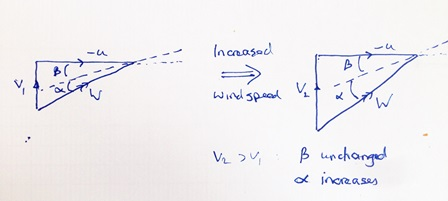
\includegraphics[width=0.85\textwidth]{./figures/angleattack}
\caption{effect of increased wind speed on angle of attack}
\label{figure:q2sol}
\end{figure}


\item \lbrack\ 3 marks ] If that happened, what could be done to reduce the angle of attack back to its original value?\par
Increase pitch angle $\beta$ or increase speed of rotation, if either are possible.
\item \lbrack\ 3 marks ] Explain why the rotor blade stalls if the angle of attack becomes too large.\par
As angle increases, laminar flow cannot be sustained beyond a critical speed, limited by air viscosity and shape of foil. Eventually, flow detaches and becomes turbulent. This means there is now no (or, less) lift on foil, since no (less) net downward motion is now imparted to fluid.
\end{enumerate}

\paragraph{\textbf{Solutions to Question 3: (13 marks)}}
A \SI{6}{\kilo\watt} wind turbine on a small holding generates \SI{10000}{\kilowatthour} per year. The household uses \SI{4000}{\kilowatthour}
per year and \SI{8000}{\kilowatthour} per year is exported. The Feed-in tariff (FiT) for this turbine when commissioned was \SI{23}{\pence\per\kilowatthour},
the export tariff was \SI{4.7}{\pence\per\kilowatthour} and the import tariff is \SI{15}{\pence\per\kilowatthour}. 
The cost of the turbine was \SI{25000}[\pounds]{}.

\begin {enumerate} [label=\alph*)]
\item \lbrack\ 3 marks ]What is the annual income from the FiT?\par
FiT income = Generated kWh x FiT tariff = $10,000\times 0.23=\SI{2300}[\pounds]{}$
\item \lbrack\ 3 marks ]By how much is the annual electricity bill of the small holding reduced because of the turbine?\par
kWh from turbine = 10,000-8000 \si{\kilowatthour}. Hence imports reduced by \SI{2000}{\kilowatthour}, so bill reduced by $2000\times0.15=\SI{300}[\pounds]{}$
\item \lbrack\ 3 marks ]Estimate the simple pay-back time of this turbine.\par
Pay back = $\dfrac{\mathrm{Capital\ expanse}}{\mathrm{Annual\ income\ +Annual\ savings}}=\dfrac{25000}{2300+8000\times0.047+300}=\SI{8.4}{\year}$
\item \lbrack\ 2 marks ]If discounting is taken into account, what impact would that have on the pay-back time as calculated in the previous part?\par
Will likely increase it, since discounting reduces present value of revenues and savings in the future.
\item \lbrack\ 2 marks ]What could the owners do to reduce this payback time?\par
Either site the turbine in windier spot, if that is possible, or better align their usage to times when wind is lowing strongly, to exploit the differential between the import and export tariffs.
\end{enumerate}


\paragraph{\textbf{Solutions to Question 4: (13 marks)}}
Wind power is widely regarded as a low-carbon source of electricity. Briefly outline the circumstances (if any) under which this is true.
A good answer will demonstrate knowledge of the actual carbon intensity of wind-produced electricity, how this compares to the carbon intensity 
of electricity from other sources and of the factors that most contribute to it.\par
Credit awareness \ discussion of 
\begin{itemize}
\item Scale as a factor - contrast with solar power
\item Reported LCA figures for wind
\item Major contributing factors (steel for towers, degree of recycling)
\item Context of carbon intensities from other renewable and non-renewable sources.
\item Use of suitable metrics (eg gCO2e/kWh; energy payback; energy yield ratio.
\item Scope for reduction eg by use of direct drive
\item Case studies/examples of LCA or metastudies.
\item Any other relevant point
\item Use of good English and grammar.
\end{itemize}


%\end{comment}

\end{document}

